\chapter{Application of Signal Processing Filters}\label{ch:AFE}
\section{Effect of Filter Characteristics on Signals}
% Therefore, smaller bandpass ripple is suggested to avoid large effect on the signal.
% filter recommendation
In the section, the effects of different filter characteristics on the rise time, time delay, and magnitude attenuation of the signals are studied. The studied filter types include Butterworth filter, Chebyshev filter and Elliptic filters. Since the Bessel filter is a pure analog filter which can not be simulated by MATLAB, its application is not included in this work. The experimented filter characteristics are given in Table~\ref{table:AFE_filterParam}. 
%
\begin{table}[]
\centering
\caption{Filter characteristics}
\label{table:AFE_filterParam}
\begin{tabular}{|l|c|l|l|}
\hline
Type & \multicolumn{1}{l|}{Butterworth} & Chebyshev & Elliptic \\ \hline
Cutoff Frequency & \multicolumn{3}{c|}{2.5 GHz} \\ \hline
Order & \multicolumn{3}{c|}{3, 5, 7} \\ \hline
Passband & - & \multicolumn{2}{c|}{3 dB, 5 dB, 10 dB} \\ \hline
Stopband & \multicolumn{2}{c|}{-} & \multicolumn{1}{c|}{30 dB} \\ \hline
\end{tabular}
\end{table}
%
In the experiment, the pulses reflected from the target were used as the signals feed into the filters. The target was set at 20m ($0.133\mu s$), and white noise arisen from electrical system was generated by the noise model and added to the return pulses. Here, we assume no other distortion or noises acts on the signal. A noise-free signal returned from the same distance was also provided as a reference signal. By comparing with the noise-free signal, the following metrics are used for the evaluation of the influence of the filter on the signals:
\begin{itemize}
  \item Rise-time difference: $\Delta t_r= t_{r, meas} - t_{r, noise-free}$, and $t_{r, noise-free}=3.55ns$;
  \item Time shift: $\Delta t_{peak} = t_{peak, meas} - t_{peak, noise-free}$, and $t_{peak, noise-free}=0.133\mu s$;
  \item Signal magnitude attenuation: $\Delta_P=\frac{P_{means}-P_{noise-free}}{P_{noise-free}}$, and $P_{noise-free} = 20.17\mu W$.
\end{itemize}
The transmit signal and its single-sided power spectrum is given in Figure~\ref{fig:AFE_transmit}, and the return signal contaminated by white noise and its power spectrum is shown in Figure~\ref{fig:AFE_return}. Figure~\ref{fig:AFE_return} shows that the return signal has a noisy spectrum at high frequencies which causes the fluctuation of the signal in time domain. 
\begin{figure}[t!p]
\centering
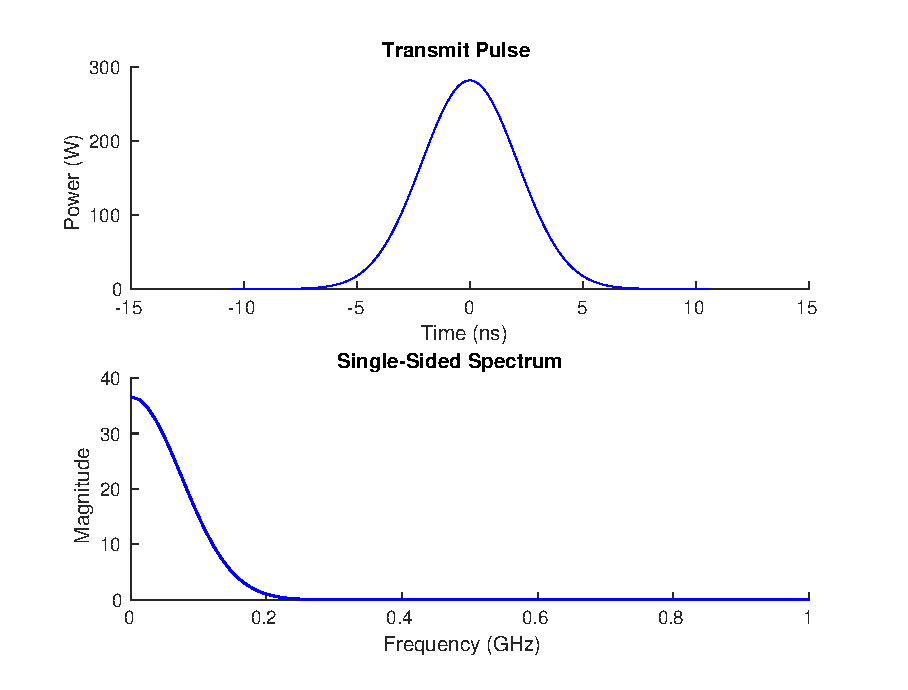
\includegraphics[width=1\textwidth]{figures/chapter_AFE/sig_start.eps}
\caption{Transmit pulse (top) and the single-sided power spectrum (bottom)}
\label{fig:AFE_transmit}
\end{figure}
%
\begin{figure}[t!p]
\centering
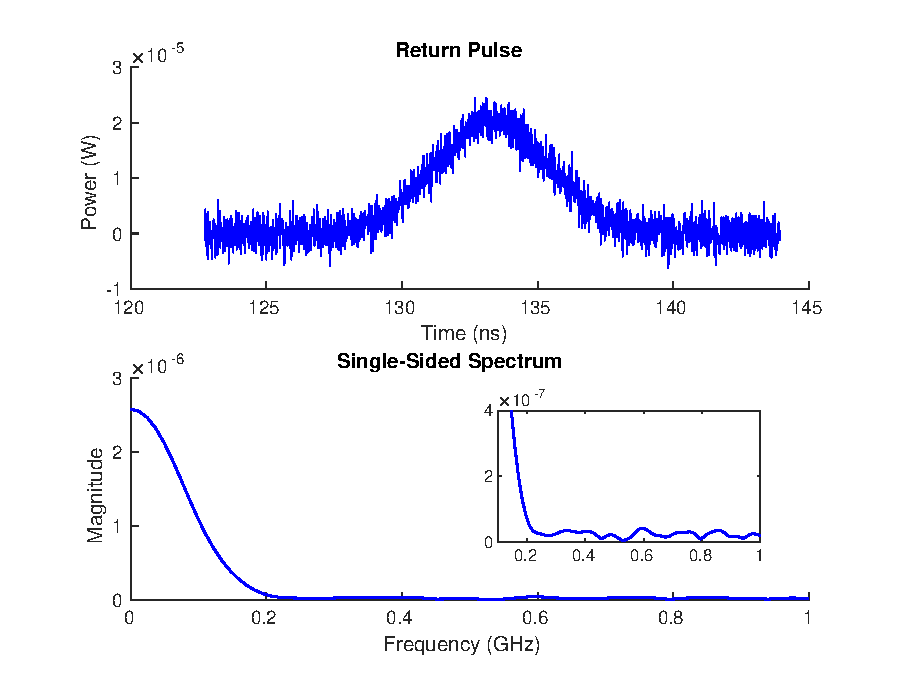
\includegraphics[width=1\textwidth]{figures/chapter_AFE/sig_return.eps}
\caption{Return pulse(top) and the single-sided power spectrum(bottom). The lower portion of the power spectrum is zoomed in and is shown in the sub-figure on the right.}
\label{fig:AFE_return}
\end{figure}
\subsection{Effect of orders}
In the study of the effect of filter order, the passband ripple of the Chebyshev and Elliptic filter was set to 3 dB and the stopband of the Elliptic filter was set to 30 dB. The effects of the order on the signal characteristics are shown in Figure~\ref{fig:AFE_res_orderEffect}. The figure demonstrates that the magnitude attenuation by the filters increases with orders for the Chebyshev and Elliptic filter. The Chebyshev filter has the largest attenuation, followed by the Elliptic filter at the same order, while the effect of the Butterworth filter is very slight. The reason is that the oscillation of the passband ripple of the Chebyshev and Elliptic filter increases with the order, as shown in the magnitude response of the two types of filters (Figure~\ref{fig:AFE_freqResp_chebyr_order}(b) and Figure~\ref{fig:AFE_freqResp_ellip_order}(b)), and the increased ripple at the passband results in larger distortion of the signal magnitude. However, the Butterworth filter has a flat passband (Figure~\ref{fig:AFE_freqResp_butter_order}(b)), so the in-band frequency components are not affected by the change of order.\par
Moreover, the rise time and time shift of the signal also changes with the order. As shown in\todo{change figure, fix ylim} Figure~\ref{fig:AFE_freqResp_butter_order}(c), Figure~\ref{fig:AFE_freqResp_chebyr_order}(c) and Figure~\ref{fig:AFE_freqResp_ellip_order}(c), the nonlinearity of the phase response increases with orders, and the Chebyshev filter has the worst linearity followed by the Elliptic filter. According to Equation~\eqref{eq:backgrnd_AFE_grouddelay}, the non-constant slope of the phase response curve causes group delay distortion of the signal which eventually alters the rise time. Moreover, since the time delay of the signal is equal to the slope of the response curve (group delay), the higher order also results in an increase of the time shift. 
\begin{figure}[h]
\centering
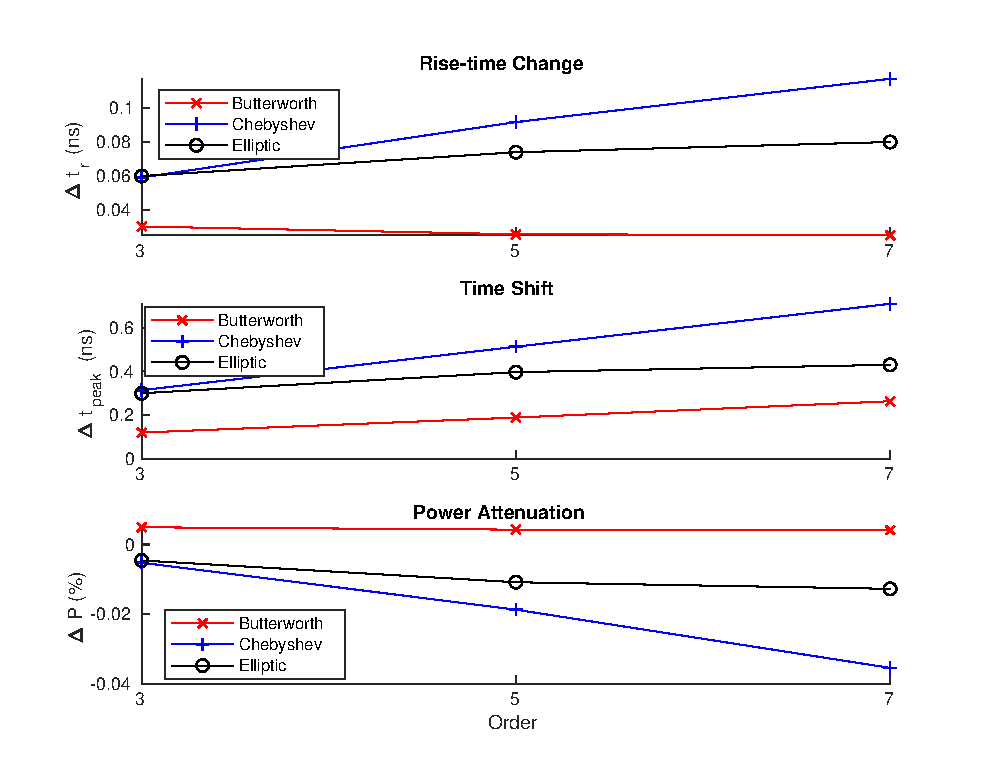
\includegraphics[width=1\textwidth]{figures/chapter_AFE/Effect_order_diff_filter.eps}
\caption{Effect of filters order on the signal characteristics}
\label{fig:AFE_res_orderEffect}
\end{figure}
\begin{figure}[t!p]
\centering
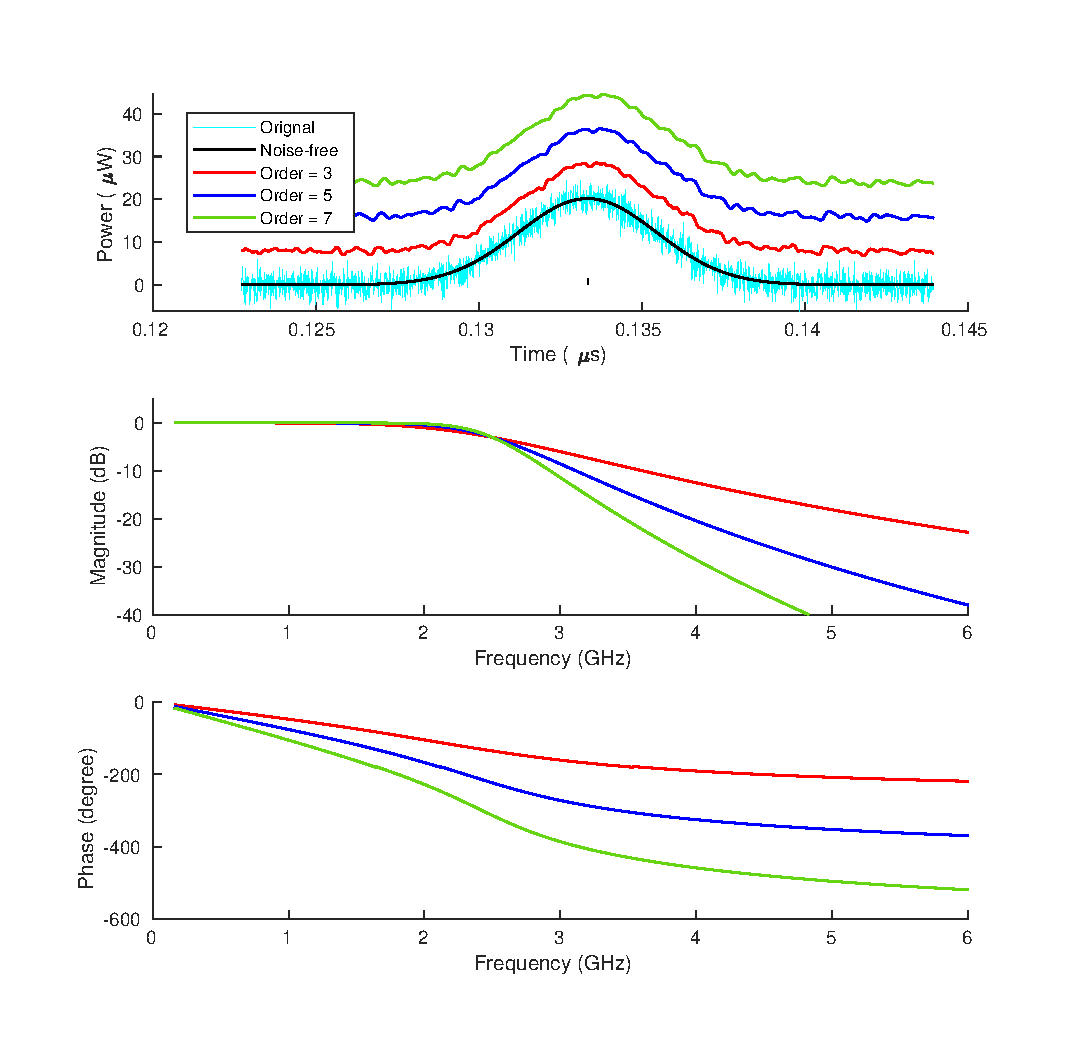
\includegraphics[width=1\textwidth]{figures/chapter_AFE/freq_response_butter_diffOrder.eps}
\caption{Frequency response of Butterworth filter with different orders}
\label{fig:AFE_freqResp_butter_order}
\end{figure}
%
\begin{figure}[t!p]
\centering
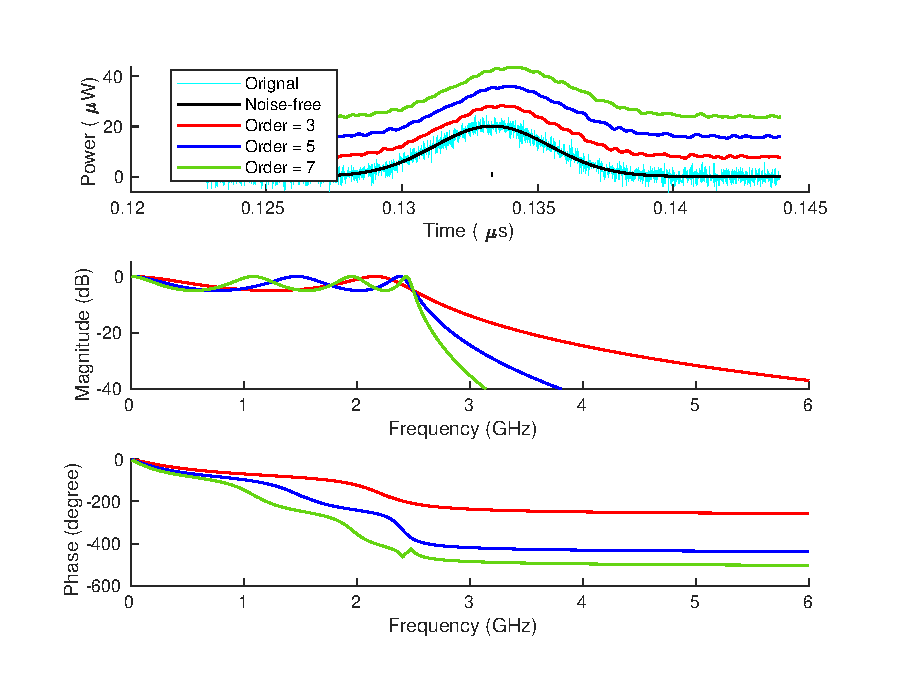
\includegraphics[width=1\textwidth]{figures/chapter_AFE/freq_response_cheby_diffOrder.eps}
\caption{Frequency response of Chebyshev filter with different orders}
\label{fig:AFE_freqResp_chebyr_order}
\end{figure}
\begin{figure}[t!p]
\centering
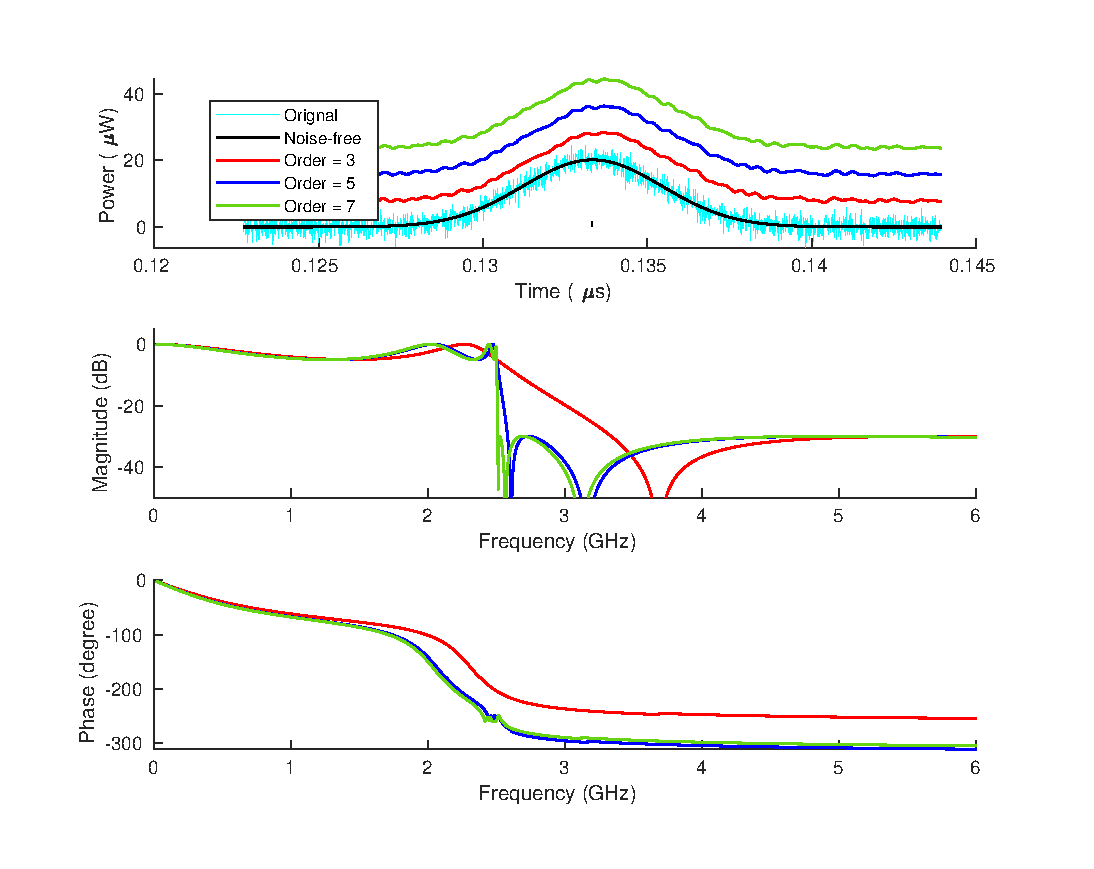
\includegraphics[width=1\textwidth]{figures/chapter_AFE/freq_response_elliptic_diffOrder.eps}
\caption{Frequency response of Elliptic filter with different orders}
\textbf{\label{fig:AFE_freqResp_ellip_order}}
\end{figure}
% Passband
\subsection{Effect of passband ripples}
The effect of passband ripples on the signal characteristics is also studied. In the study, to control the number of variables, the order of all the filters was set to 3 and the stopband ripple of the Elliptic filter remains 30 dB. The signal characteristics after filtering by filters with different passband ripples are presented in Figure~\ref{fig:AFE_res_rppassEffect}, and the results of the Butterworth filter are also provided for comparison. The frequency response of the Chebyshev and Elliptic filter are shown in Figure~\ref{fig:AFE_freqResp_cheby_pass} and Figure~\ref{fig:AFE_freqResp_ellip_pass}.As discussed before, high passband ripple causes a larger magnitude distortion of the signal, resulting in an increase of power attenuation. Furthermore, as the ripple value increases, the phase response becomes more nonlinear, which results in a larger change of rise time and the time shift of the signal. 
%
\begin{figure}[t!p]
\centering
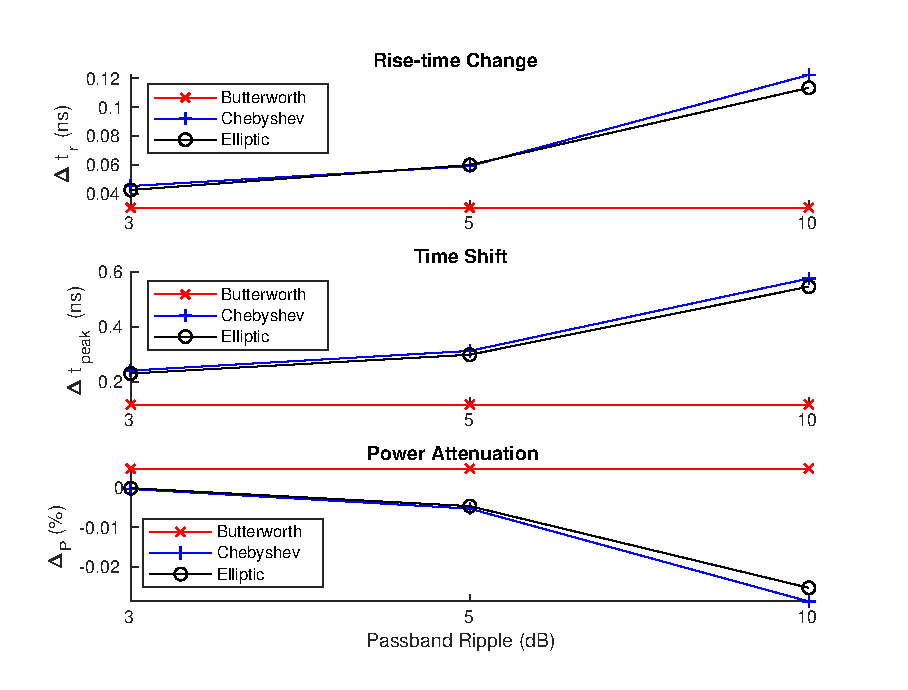
\includegraphics[width=1\textwidth]{figures/chapter_AFE/Effect_rppass_diff_filter.eps}
\caption{Effect of passband ripple order on the signal characteristics}
\label{fig:AFE_res_rppassEffect}
\end{figure}
%
\begin{figure}[t!p]
\centering
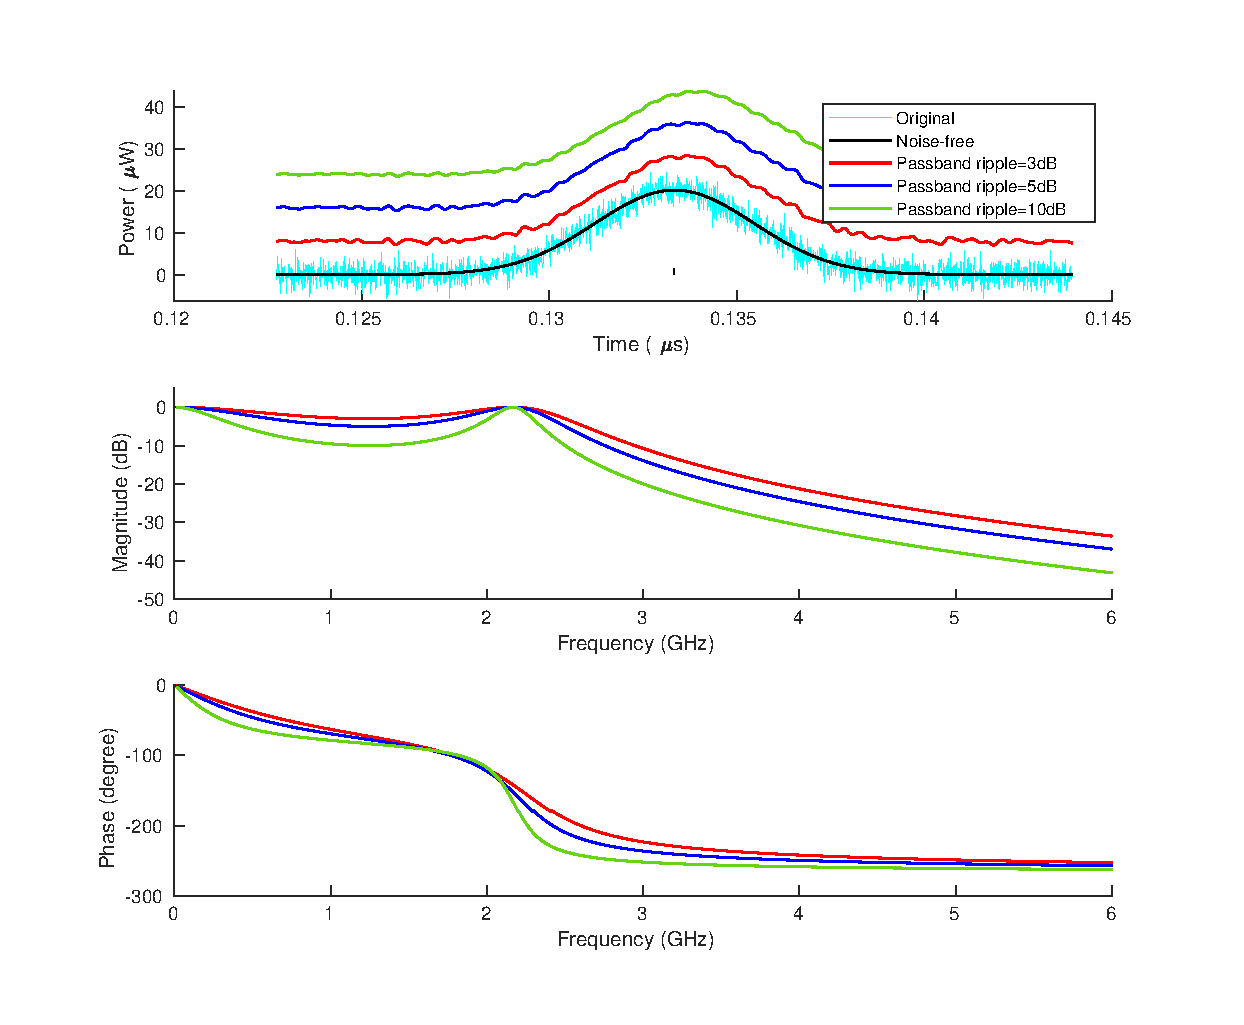
\includegraphics[width=1\textwidth]{figures/chapter_AFE/freq_response_cheby_diffPass.eps}
\caption{Frequency response of Chebyshev filter with different passband ripples}
\label{fig:AFE_freqResp_cheby_pass}
\end{figure}
%
\begin{figure}[t!p]
\centering
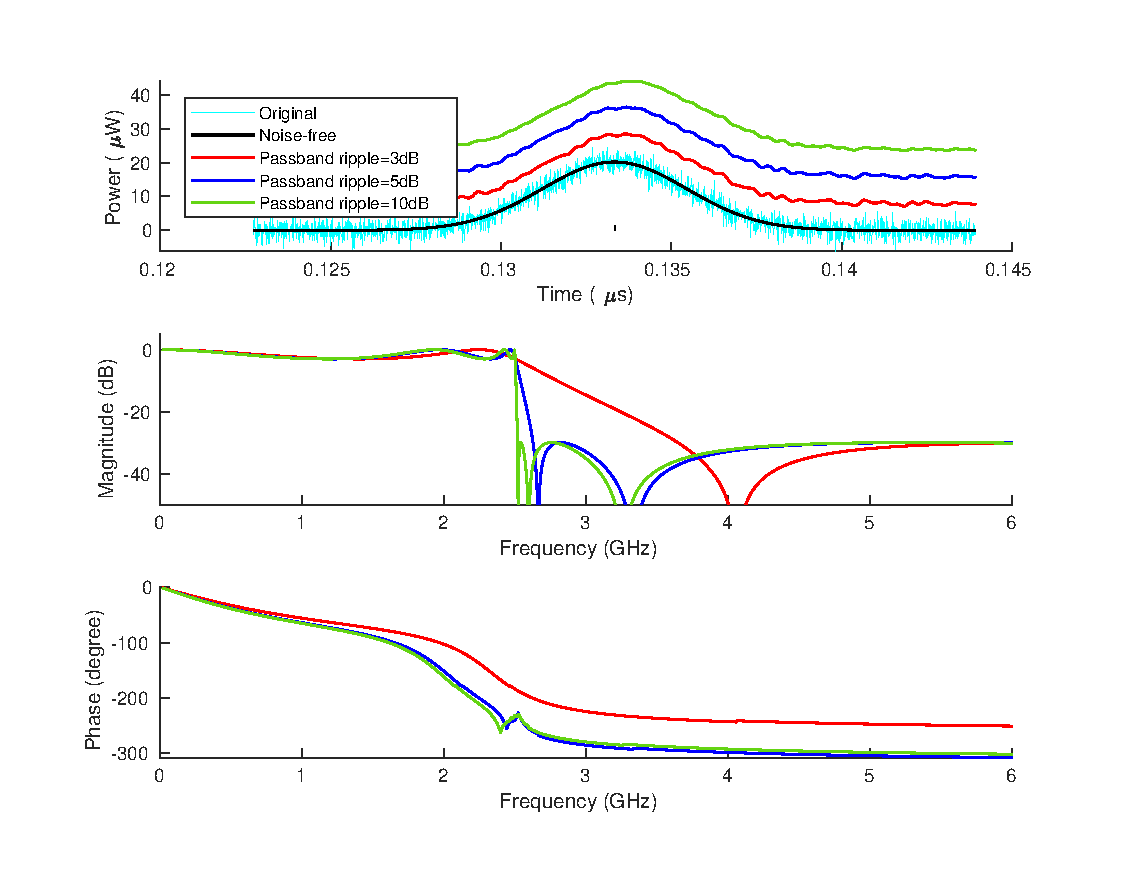
\includegraphics[width=1\textwidth]{figures/chapter_AFE/freq_response_elliptic_diffPass.eps}
\caption{Frequency response of Elliptic filter with different passband ripples}
\textbf{\label{fig:AFE_freqResp_ellip_pass}}
\end{figure}

%% filtfilt
\subsection{Zero-phase filtering}
From the above discussion, we can see the application of filters with nonlinear phase response will cause an increase of rise time and a time delay of the signal. The enlarged rise time and time shift could cause biased distance measurement and increased measurement uncertainty. To reduce the impact on the rise time, one solution is to apply a filter with linear phase response, and the Bessel filter is a desired but the trade-off is that the roll-off of the filter is slower than the Chebyshev and Elliptic filters. To address the time shift, one approach is to apply a filter to both START signal and STOP signal sensed by the receiver. Therefore, the time delay at the two signals are cancelled in the TOF calculation. If in any case no filter is applied to one of the signal, the time delay arisen from the filter can also be calibrated from experiments and be subtracted from the calculated TOF. Additionally, an all-pass filter with a customized phase response according to the time delay can also be added after the original filter to compensate the group delay.\par
In the signal processing, the \emph{zero-phase filtering} can compensate the time shift caused by the filter and provide zero-phase shift. Generally, a signal is only feed into the filter once, which is called ‘forward filtering’. However, the zero-phase filtering has additional step that feeds the signal backwards after the forward filtering. Since backwards filtering causes a negative group delay, the positive and negative group delays are canceled and a zero-phase signal is achieved. The zero-phase filtering can be performed by using any aforementioned type of filters. The effect of the zero-phase filtering on the signal characteristics is also studied in this work. The filtered signals and the resultant characteristics are given in Figure:\ref{fig:AFE_filtfilt} and Table~\ref{table:AFE_res_phaseComp}. In the experiment, the cutoff frequency of the filters was set to 1 GHz, the order of the filters set to 3, the passband ripple 3 dB and stopband ripple 30 dB. From the results we can see the time shift is theoretically eliminated. However, the power attenuation caused the Chebyshev and Elliptic filter is doubled, and rise-time difference also becomes worse. The reason for those effects is that the zero-phase filter actually filters a signal twice, so the distortion of the signal is worsen than the forward filtering. In our case, the signals were actually filtered by filters with a passband ripple of 6 dB. On the other hand, since the Butterworth filter has a flat passband, the distortion caused by Butterworth filter is much less than the other two. Another drawback of the zero-phase filtering is that the entire signal should be available for the zero-phase filtering, which means the zero-phase filtering can not be realized in real-time by an analog circuit but can only be performed offline. Therefore, even though the zero-phase is powerful of removing the time-shift of the signal, it is only limited to offline post-processing signals that are stored beforehand. 
%
\begin{figure}[t!p]
\centering
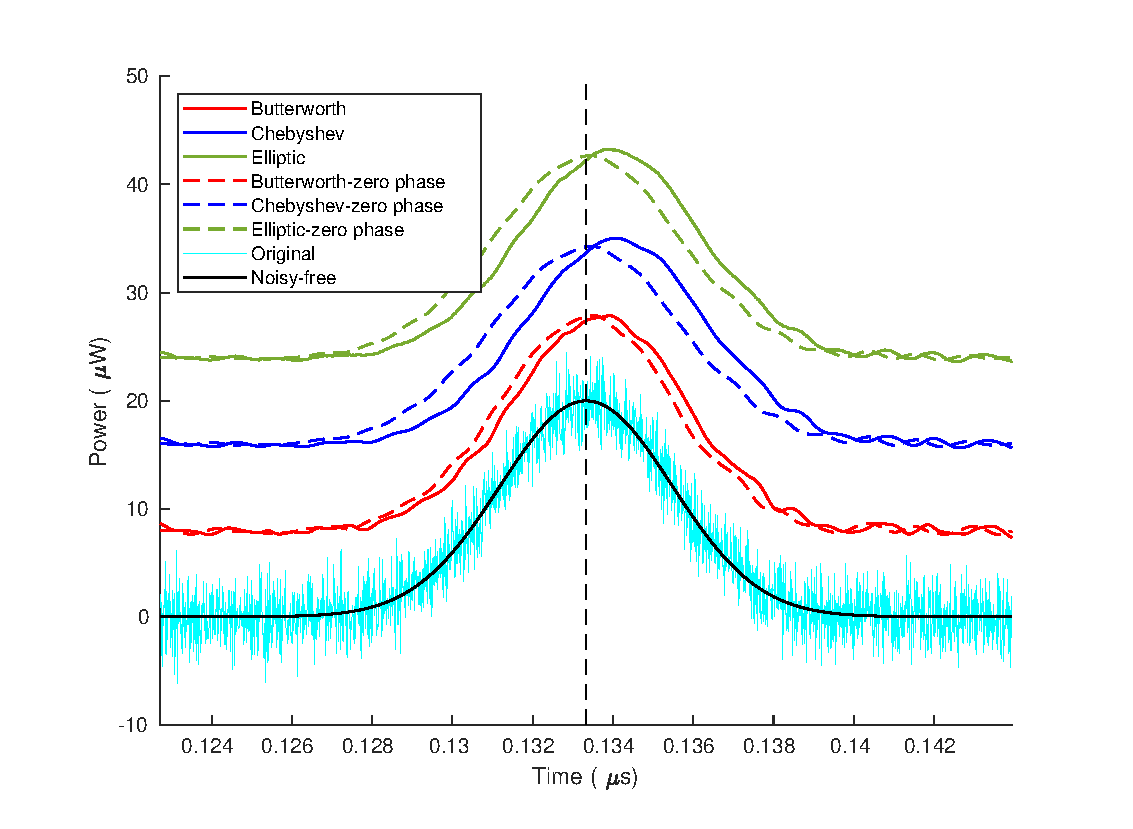
\includegraphics[width=1\textwidth]{figures/chapter_AFE/sig_filtfilt.eps}
\caption{Signal after phase-shift compensation}
\label{fig:AFE_filtfilt}
\end{figure}
%
\begin{table}[h]
\centering
\caption{Result of signal characteristics after phase-shift compensation}
\label{table:AFE_res_phaseComp}
\begin{tabular}{|l|c|c|c|c|c|c|}
\hline
Filter Type & \multicolumn{2}{c|}{Butterworth} & \multicolumn{2}{c|}{Chebyshev} & \multicolumn{2}{c|}{Elliptic} \\ \hline
Phase shift compensation & No & \multicolumn{1}{l|}{zero-phase} & No & \multicolumn{1}{l|}{zero-phase} & No & \multicolumn{1}{l|}{zero-phase} \\ \hline
Rise-time Difference (ns) & 0.042 & 0.037 & 0.061 & 0.218 & 0.061 & 0.196 \\ \hline
Time Shift (ns) & 0.632 & -0.015 & 0.750 & -0.030 & 0.726 & -0.030 \\ \hline
Power Attenuation ratio (\%) & 0.010 & -0.104 & -2.045 & -4.022 & -1.984 & -3.907 \\ \hline
\end{tabular}
\end{table}



%%
% application of filters with different params to sim signals --> Butter is best
% applicadton o filters to real signal, compare w/o filt and w/ filt. -> ADC MF


%%\subsection{Digital Filters}

%% filter implementation: LP filter can attenuate the signal amplitude if fcut is inside the BW: [Figure 4, Challenges in miniaturized automotive long-range lidar system design]
